\documentclass[11pt]{article}
\usepackage[margin=1in]{geometry}
\usepackage{amsmath,amssymb,amsthm,mathtools}
\usepackage{graphicx}
\usepackage{microtype}
\usepackage{enumitem}
\usepackage{xcolor}
\usepackage[colorlinks=true,linkcolor=blue!55!black,citecolor=blue!55!black,urlcolor=blue!55!black]{hyperref}

\newtheorem{theorem}{Theorem}
\newtheorem{lemma}{Lemma}
\newcommand{\1}{\mathbf 1}
\newcommand{\R}{\mathbb R}
\newcommand{\N}{\mathbb N}
\newcommand{\Borel}{\mathcal B}
\newcommand{\esssup}{\mathop{\rm ess\,sup}}

\title{Two Counterexamples for Normalized Separating Hyperplanes\\
\large Negative answers to both open questions on page 7 of arXiv:1508.05249}
\author{Automated mathematics run \texttt{fa\_banach\_001}, lane 10}
\date{11 August 2026}

\begin{document}
\maketitle

\begin{center}
\fbox{\parbox{0.91\textwidth}{\textbf{Status.} Candidate counterexample,
likely valid, pending human mathematical review.  Both conclusions below are
proved analytically; the included code is supplementary verification only.}}
\end{center}

\section{Source questions and answer}

Steinwart's paper \cite{Steinwart2015} studies a continuous functional
$\Gamma:B\to\R$ on a convex subset of a normed space and the unique normalized
functionals separating its level sets.  On PDF page 7 it asks:

\begin{quote}
``Finally, whether $r\mapsto h_r$ is actually measurable with respect to
$L_\infty(\mu)$ remains an open question.''
\end{quote}

After proving that the weak level-set continuity condition G5 is automatic in
finite dimensions, the paper also asks:

\begin{quote}
``Whether this is true in more general settings remains an open question.''
\end{quote}

The source passages are reproduced below at full text width.

\begin{figure}[ht]
  \centering
  
\includegraphics[width=\textwidth]{figures/open_problem_crop.png}
  \caption{The $L^\infty$-measurability question, source PDF page 7.}
\end{figure}

\begin{figure}[ht]
  \centering
  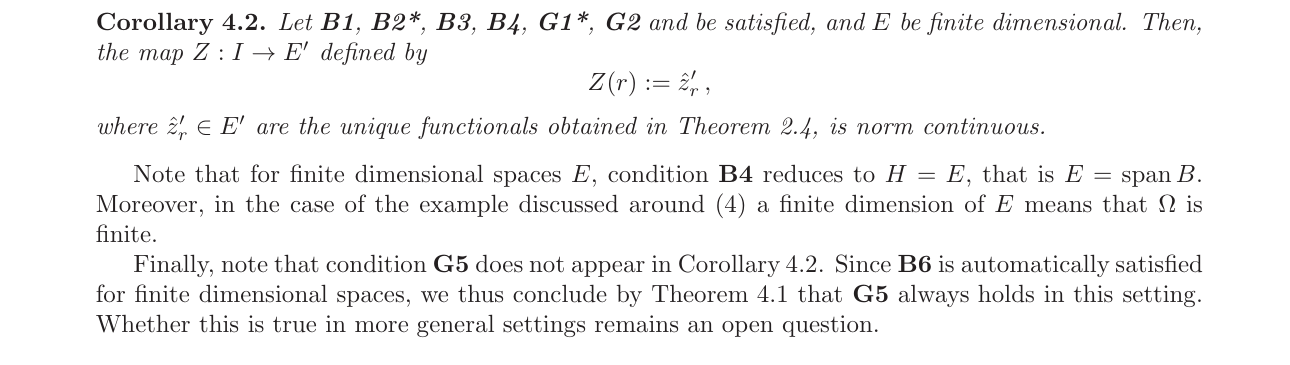
\includegraphics[width=\textwidth]{figures/open_problem_g5_crop.png}
  \caption{The G5 question and its finite-dimensional context, source PDF page 7.}
\end{figure}

We answer both questions negatively, inside the motivating model of bounded
probability densities.  The first example has a continuous, strictly
quasi-monotone property but fails G5.  The second has normalized representatives
which are continuous in every finite $L^p$ but are not even norm-Borel
measurable in $L^\infty$.

\section{Framework from the source paper}

Let $(\Omega,\mathcal A,\mu)$ be a probability space,
\[
 E=L^1(\mu),\qquad
 B=\{p\in L^\infty(\mu):p\geq0,\ \textstyle\int p\,d\mu=1\}.
\]
This is exactly the bounded-density set in equation (4) of
\cite{Steinwart2015}.  We use its standard facts, spelling them out because
they are essential to the counterexamples.

Take $p_\star=\1$.  Then $H=\operatorname{span}B=L^\infty(\mu)$ and
\[
 F=\operatorname{span}(-p_\star+B)
   =\{f\in L^\infty(\mu):\textstyle\int f\,d\mu=0\}.
\]
With $\|\cdot\|_F=\|\cdot\|_\infty$, the $F$-norm dominates the $L^1$-norm
and $0$ is an interior point of $-p_\star+B$ in $F$.  Thus B1 and B2* hold.
Positive and negative parts give B3 (with $K=1$ for the $L^1$ norm), and
density of $L^\infty$ in $L^1$ gives B4.

For a family $\phi_r\in L^\infty(\mu)$, suppose that for every $p\in B$ the
scalar function
\[
 F_p(r):=\int \phi_r p\,d\mu
\]
is continuous, strictly monotone, and has a unique zero.  Denote that zero by
$\Gamma(p)$.  Then
\[
 \{\Gamma=r\}=\{p\in B:F_p(r)=0\}
\]
is convex.  Moreover, if $\Gamma(p)=u<v=\Gamma(q)$, every nontrivial convex
mixture of $p$ and $q$ has its zero strictly between $u$ and $v$.  Therefore
$\Gamma$ is quasi-monotone and is strictly quasi-monotone on the interior of
its image.  Once continuity is verified, Theorem 2.4 of
\cite{Steinwart2015} shows that G1* and G2 hold and identifies the unique
normalized separating functionals.

\section{Proof intuition}

Normalization is the only source of pathology in the first example.  We make
unnormalized separators $z_r$ converge weak-star as $r\downarrow r_0$, while a
``bump escaping to infinity'' keeps $\|z_r\|_\infty$ large for every $r>r_0$.
At $r_0$ that bump disappears pointwise and the norm drops.  Dividing by the
norm therefore changes the weak-star limit by a nontrivial scalar.  The source
paper's equivalence between G5 and weak-star continuity then gives failure of
G5.

For measurability, moving threshold functions are ideal: changing the threshold
on a short interval is small in every finite $L^p$, but its $L^\infty$ size is
unchanged.  After normalization, any two distinct thresholds remain more than
one apart in $L^\infty$.  Open unions of disjoint balls can consequently encode
arbitrary subsets of the parameter interval, including nonmeasurable ones.

\section{Main result}

\begin{theorem}[Full negative answers]\label{thm:main}
The following statements hold.
\begin{enumerate}[label=\textup{(\Alph*)}]
\item There exist a probability space, $E=L^1(\mu)$, the bounded-density set
  $B$ above, and an $L^1$-continuous functional $\Gamma:B\to\R$ satisfying
  B1, B2*, B3, B4, B6, G1*, and G2, for which G5 fails.
\item There exist an atomless probability space and such a functional
  $\Gamma$ for which the unique normalized representing curve
  $r\mapsto h_r\in L^\infty(\mu)$ is not measurable from the completed
  Lebesgue sigma-algebra on $I$ to the norm-Borel sigma-algebra of
  $L^\infty(\mu)$.  Nevertheless, it is continuous as an $L^p$-valued map
  for every $1\leq p<\infty$.  The auxiliary-space hypotheses of Corollary
  3.2 in \cite{Steinwart2015} hold with $E_0=L^2(\mu)$.
\end{enumerate}
\end{theorem}

\section{A continuous property for which G5 fails}

Let $\Omega=\N$, let $\mu(\{k\})=2^{-k}$, and use the bounded-density model
above.  Then $E=L^1(\mu)$ is an infinite-dimensional separable Banach space,
so B6 holds.  Set
\[
 r_0=\frac12,\qquad \delta=\frac1{16},\qquad \varepsilon=\frac14,
\]
and
\[
 a_1=r_0+\delta,\qquad a_2=r_0-\delta,\qquad a_k=r_0\quad(k\geq3).
\]
For $r\in\R$ and $k\in\N$, define
\[
 q_r(k)=
 \begin{cases}
 0,&r\leq r_0,\\
 \min\{1,(r-r_0)k\},&r>r_0,
 \end{cases}
 \qquad
 \phi_r(k)=r-a_k+\varepsilon q_r(k).
\]
For $p\in B$, put $F_p(r)=\int\phi_rp\,d\mu$.

\subsection{The root functional satisfies the source hypotheses}

For fixed $k$, $r\mapsto q_r(k)$ is continuous and nondecreasing.  Dominated
convergence therefore gives continuity of $F_p$, and for $s>r$,
\[
 F_p(s)-F_p(r)
  =(s-r)+\varepsilon\int(q_s-q_r)p\,d\mu\geq s-r.
\]
Thus $F_p$ is strictly increasing.  At $r_0-\delta$, every coordinate of
$\phi_r$ is nonpositive; at $r_0+\delta$, every coordinate is nonnegative and
the $q_r$ term is strictly positive.  Hence
\[
 F_p(r_0-\delta)\leq0<F_p(r_0+\delta),
\]
so $F_p$ has a unique zero in $[r_0-\delta,r_0+\delta)$.  Define
$\Gamma(p)$ to be this zero.

The functional is $L^1$-continuous.  Indeed, if
$u=\Gamma(p)<v=\Gamma(q)$, then
\[
 v-u\leq F_p(v)-F_p(u)=F_p(v)
 =\int\phi_v(p-q)\,d\mu
 \leq \|\phi_v\|_\infty\|p-q\|_1.
\]
On the root interval $\|\phi_v\|_\infty\leq2\delta+\varepsilon$, giving a
uniform Lipschitz bound (and the case $v<u$ is symmetric).

Let $p^{(j)}=\mu(\{j\})^{-1}\1_{\{j\}}$.  Direct calculation gives
\[
 \Gamma(p^{(2)})=r_0-\delta,
 \qquad
 \Gamma(p^{(1)})=r_0+\frac{\delta}{1+\varepsilon}.
\]
Since $B$ is convex and $\Gamma$ is continuous, the interior $I$ of
$\Gamma(B)$ contains $r_0$ and a right-neighborhood of $r_0$.

Level sets are affine sections because
$\{\Gamma=r\}=\{p:F_p(r)=0\}$.  If
$\Gamma(p)=u<v=\Gamma(q)$ and $0<\theta<1$, then, for
$m=(1-\theta)p+\theta q$,
\[
 F_m(u)=\theta F_q(u)<0,
 \qquad
 F_m(v)=(1-\theta)F_p(v)>0.
\]
Thus $u<\Gamma(m)<v$.  This proves strict quasi-monotonicity on $B$, hence in
particular on $\Gamma^{-1}(I)$.  Theorem 2.4 of \cite{Steinwart2015}, together
with the already verified B-assumptions and continuity, yields G1* and G2.

\subsection{Normalization breaks weak-star continuity}

Because $F_p$ is increasing, the correctly oriented separator is
$z_r=-\phi_r$: one has $\Gamma(p)<r$ exactly when
$\langle z_r,p\rangle<0$.  The unique normalized separator is therefore
\[
 \widehat z_r=\frac{z_r}{\|z_r\|_\infty}\in(L^1(\mu))'=L^\infty(\mu).
\]
At $r=r_0$,
\[
 z_{r_0}=(\delta,-\delta,0,0,\ldots),
 \qquad \|z_{r_0}\|_\infty=\delta.
\]
Now let $t>0$ be small.  On sufficiently large coordinates $k$ we have
$tk\geq1$, hence $|z_{r_0+t}(k)|=\varepsilon+t$.  The first two coordinates
are
\[
 \phi_{r_0+t}(1)=-\delta+(1+\varepsilon)t,
 \qquad
 \phi_{r_0+t}(2)=\delta+(1+2\varepsilon)t,
\]
and all remaining coordinates have absolute value at most $\varepsilon+t$.
For all sufficiently small $t$ these observations give the exact norm
\[
 \|z_{r_0+t}\|_\infty=\varepsilon+t.
\]

For each fixed $k$, $q_{r_0+t}(k)\to0$ as $t\downarrow0$.  The family is
uniformly bounded, so dominated convergence against every $x\in L^1(\mu)$
gives
\[
 z_{r_0+t}\overset{w^*}{\longrightarrow}z_{r_0}.
\]
Consequently,
\[
 \widehat z_{r_0+t}
 \overset{w^*}{\longrightarrow}
 \frac{z_{r_0}}{\varepsilon}
 =\frac{\delta}{\varepsilon}\widehat z_{r_0}
 =\frac14\widehat z_{r_0}
 \neq\widehat z_{r_0}.
\]
Choose, for example, $t_n=\delta/(4n)$.  The preceding image calculation
ensures $r_0+t_n\in I$.  Thus the normalized separator curve is not weak-star
continuous at $r_0$.  All hypotheses of Theorem 4.1 in
\cite{Steinwart2015} are satisfied, and that theorem states that G5 is
equivalent to weak-star continuity of this curve.  Hence G5 fails.  This proves
Theorem \ref{thm:main}(A).

\section{Finite-\texorpdfstring{$L^p$}{Lp} continuity but failure of
\texorpdfstring{$L^\infty$}{L-infinity} measurability}

Let $\Omega=(0,1)$ with Lebesgue probability measure.  For $0\leq r\leq1$ set
\[
 \phi_r(t)=1-2\1_{(0,r]}(t)-r,
 \qquad
 F_p(r)=\int_0^1\phi_r(t)p(t)\,dt
       =1-r-2\int_0^r p(t)\,dt.
\]
For every $p\in B$, $F_p$ is continuous,
$F_p(0)=1$, $F_p(1)=-2$, and, for $s>r$,
\[
 F_p(s)-F_p(r)=-(s-r)-2\int_r^s p(t)\,dt\leq-(s-r).
\]
It therefore has a unique zero; again call it $\Gamma(p)$.

Every $r\in(0,1)$ occurs as a zero.  Indeed, the bounded density
\[
 p_r(t)=
 \begin{cases}
 \dfrac{1-r}{2r},&0<t<r,\\[4pt]
 \dfrac{1+r}{2(1-r)},&r<t<1
 \end{cases}
\]
has total mass one and $\int_0^r p_r=(1-r)/2$, hence
$\Gamma(p_r)=r$.  Thus $\Gamma(B)=(0,1)$ and $I=(0,1)$.

If $u=\Gamma(p)<v=\Gamma(q)$, monotonicity gives
\[
 v-u\leq |F_p(v)-F_q(v)|
 \leq \|\phi_v\|_\infty\|p-q\|_1
 <2\|p-q\|_1.
\]
So $\Gamma$ is $L^1$-Lipschitz.  The same two-endpoint argument used above,
with inequalities reversed because $F_p$ is decreasing, shows strict
quasi-monotonicity.  Hence the source paper's G1* and G2 conditions hold.

Here the separator already has the correct orientation: $z_r=\phi_r$, and
\[
 \|z_r\|_\infty=1+r,
 \qquad
 h_r:=\widehat z_r=
 \begin{cases}
 -1,&0<t\leq r,\\[2pt]
 c_r:=\dfrac{1-r}{1+r},&r<t<1.
 \end{cases}
\]
If $0<r<s<1$, then on $(r,s]$ the two functions take the values $c_r$ and
$-1$.  Elsewhere their difference is no larger, so
\[
 \|h_r-h_s\|_\infty=1+c_r=\frac{2}{1+r}>1.\tag{1}
\]
Thus the image is an uncountable set whose distinct points are separated by
more than one.

For any subset $A\subset I$, let
\[
 U_A=\bigcup_{r\in A}B_{L^\infty}(h_r,1/2).
\]
This is open in the norm topology of $L^\infty$.  By (1),
\[
 \{s\in I:h_s\in U_A\}=A.
\]
Choose $A$ outside the completed Lebesgue sigma-algebra on $I$.  Then the
inverse image of the norm-open set $U_A$ is not measurable.  Hence
$r\mapsto h_r$ is not norm-Borel measurable and, a fortiori, is not Bochner
measurable.

This failure is invisible in every finite $L^p$.  For $1\leq p<\infty$ and
$r<s$, direct integration gives
\[
 \|h_r-h_s\|_p^p
 =(s-r)\left(\frac{2}{1+r}\right)^p
 +(1-s)|c_r-c_s|^p\longrightarrow0
 \quad(s\to r).
\]
The analogous formula from the left proves $L^p$-continuity on all of $I$.

Finally, this is within the precise auxiliary-space setting of Corollary 3.2
of \cite{Steinwart2015}.  Take $E_0=L^2(0,1)$, continuously embedded in
$L^1(0,1)$.  It is a separable Hilbert space, $B\subset L^\infty\subset L^2$,
and the B2--B4 verification above works with the same $L^\infty$ dominating
norm.  Moreover, $B$ is Borel in $L^2$: it is the intersection of the closed
positive cone and the closed integral-one hyperplane with
\[
 L^\infty=\bigcup_{m=1}^\infty\{f\in L^2:|f|\leq m\ \text{a.e.}\},
\]
whose displayed pieces are $L^2$-closed.  Thus G4 and B5 hold, and
$L^1$-Lipschitz continuity implies $L^2$-continuity.  This proves Theorem
\ref{thm:main}(B).

\section{Verification and limitations}

The included script
\texttt{code/check\_counterexamples.py} deterministically checks 80 sampled
discrete densities, 80 exact separator scales, 100 threshold levels, all
pairwise $L^\infty$ gaps on that grid, the explicit witnessing densities, and
finite-$L^p$ limits.  It prints
\begin{verbatim}
PASS: both counterexample sanity suites completed
  example A: 80 random densities and 80 separator scales
  example B: 100 levels, pairwise L-infinity separation, finite-Lp limits
\end{verbatim}
These computations are sanity checks only; no finite computation proves the
theorem.

The first counterexample uses Theorems 2.4 and 4.1 of the source paper for the
equivalence with G2 and G5.  The second conclusion is specifically about the
norm-Borel structure of $L^\infty$, the Banach-valued/Bochner interpretation
used in the source's Theorem 3.1 and the surrounding question.  Its curve is
in fact weak-star continuous, so the packet makes no claim against weak-star
measurability.

\section{Novelty check and review recommendation}

On 11 August 2026, bounded searches covered the run registry, solution index,
and attempt index, plus open web/arXiv searches for the arXiv id, exact title,
author, the exact question phrases, ``weak level set continuity,'' ``G5,'' and
close $L^\infty$-measurability variants.  They found the source paper but no
later paper explicitly answering either question.  This is bounded negative
evidence, not an exhaustive novelty claim.

The packet is recommended for high-priority human review as a candidate full
counterexample.  The principal audit points are the invocation of Theorem 2.4
after strict quasi-monotonicity, the norm computation in the escaping-coordinate
example, and the arbitrary-open-union argument in $L^\infty$.

\begin{thebibliography}{9}
\bibitem{Steinwart2015}
Ingo Steinwart,
\emph{Representation of Quasi-Monotone Functionals by Families of Separating
Hyperplanes}, arXiv:1508.05249v1 [math.OC], 2015.
\url{https://arxiv.org/abs/1508.05249}.
\end{thebibliography}

\end{document}
